\documentclass[12pt]{exam}

\usepackage[brazil]{babel}
\usepackage{enumerate}
\usepackage[utf8]{inputenc}
\usepackage{graphicx}

\extraheadheight{3cm}
\extrafootheight{2cm}
\extrawidth{2cm}
\headrule
\lhead {Universidade Estadual de Campinas 
    \\ Instituto de Computação 
    \\ \bfseries MO620 - Engenharia de Software II - Turma B 
    \\ \textnormal{Aluno: Luiz Alberto Ferreira Gomes}}
\rhead{
    Padrões de Projeto: Caixa Automático 
    \\  RA:007275}
\footrule
\footer{}{Página \thepage\ of \numpages}{}
\renewcommand{\solutiontitle}{\noindent\textbf{Solução:}\enspace}

\printanswers

\begin{document}
    Considere o Sistema de Caixa Automático descrito no capítulo 6 da apostila, e aplique os
    padrões abaixo:
    
    \begin{questions}
	
      \question Padrão de Projeto \textit{Singleton}: aplique esse padrão para garantir que a classe de controle
      tenha uma instância única.  
      \begin{solution}
        A classe do Padrão \textit{Singleton} está destacada em azul.
        
        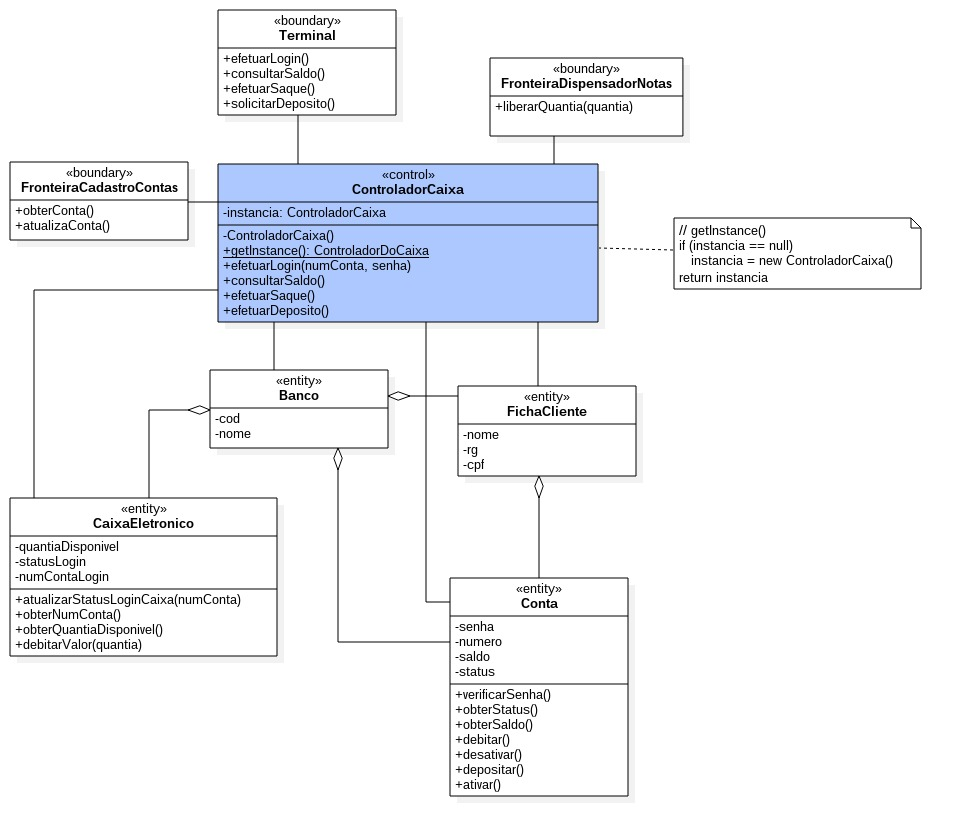
\includegraphics[width=0.85\textwidth]{imagens/lista2e1.jpg}
      \end{solution}
\pagebreak
      \question Padrão de Projeto \textit{State}: aplique esse padrão considerando que uma conta pode estar ativa
      ou inativa. No caso de uma conta estar inativa, a operação \verb!debitar()! não deve funcionar.
      \begin{solution}
         As classes do Padrão \textit{State} estão destacadas em verde.
         
        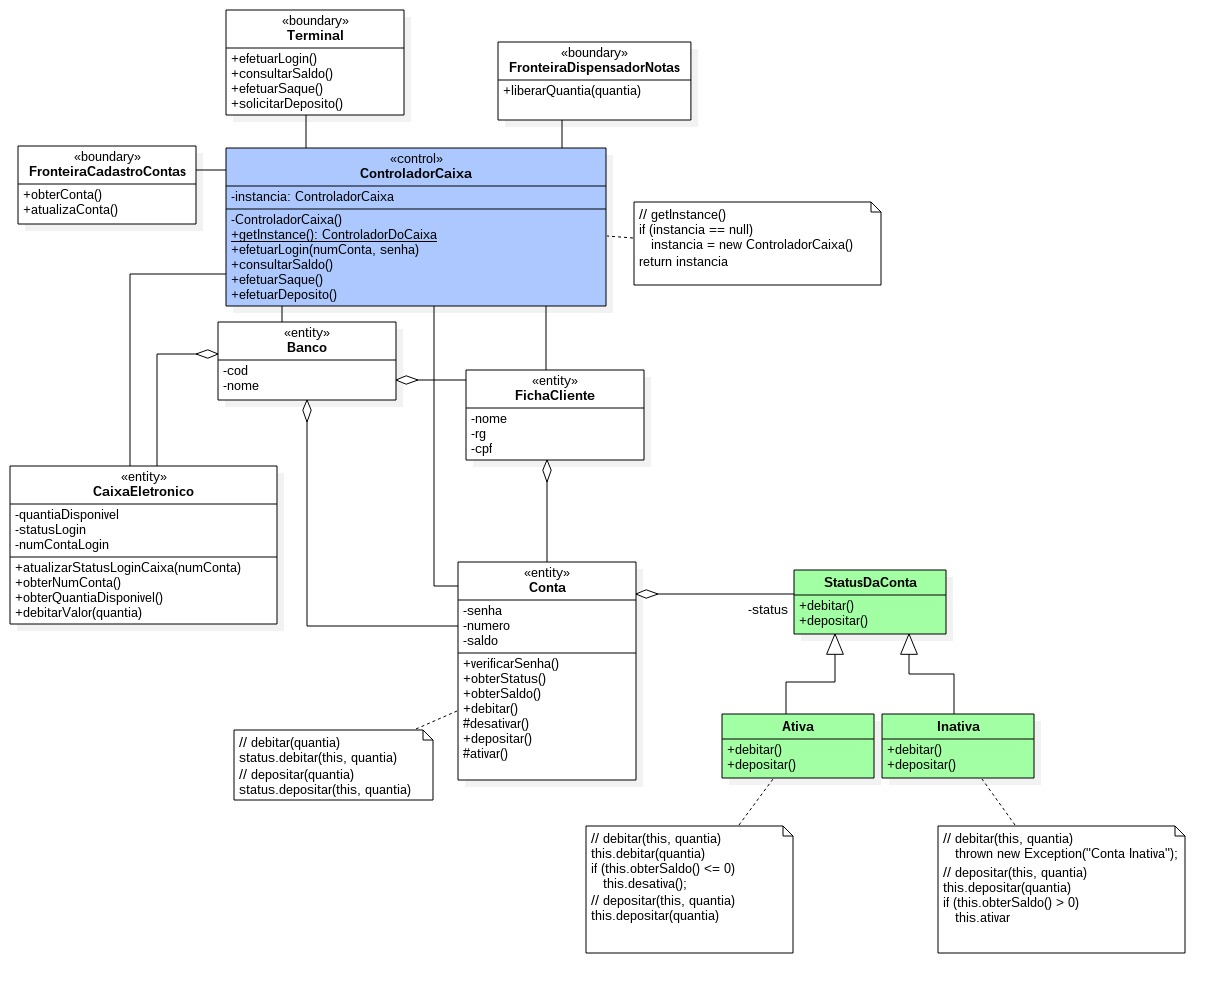
\includegraphics[width=0.92\textwidth]{imagens/lista2e2.jpg}
      \end{solution}
\pagebreak	
      \question Padrão de Projeto \textit{Factory Method}: aplique esse padrão para criar uma fábrica de tipos diferentes 
      de contas.
      \begin{solution}
        As classes do Padrão \textit{Factory Method} estão destacadas em laranja.
        
        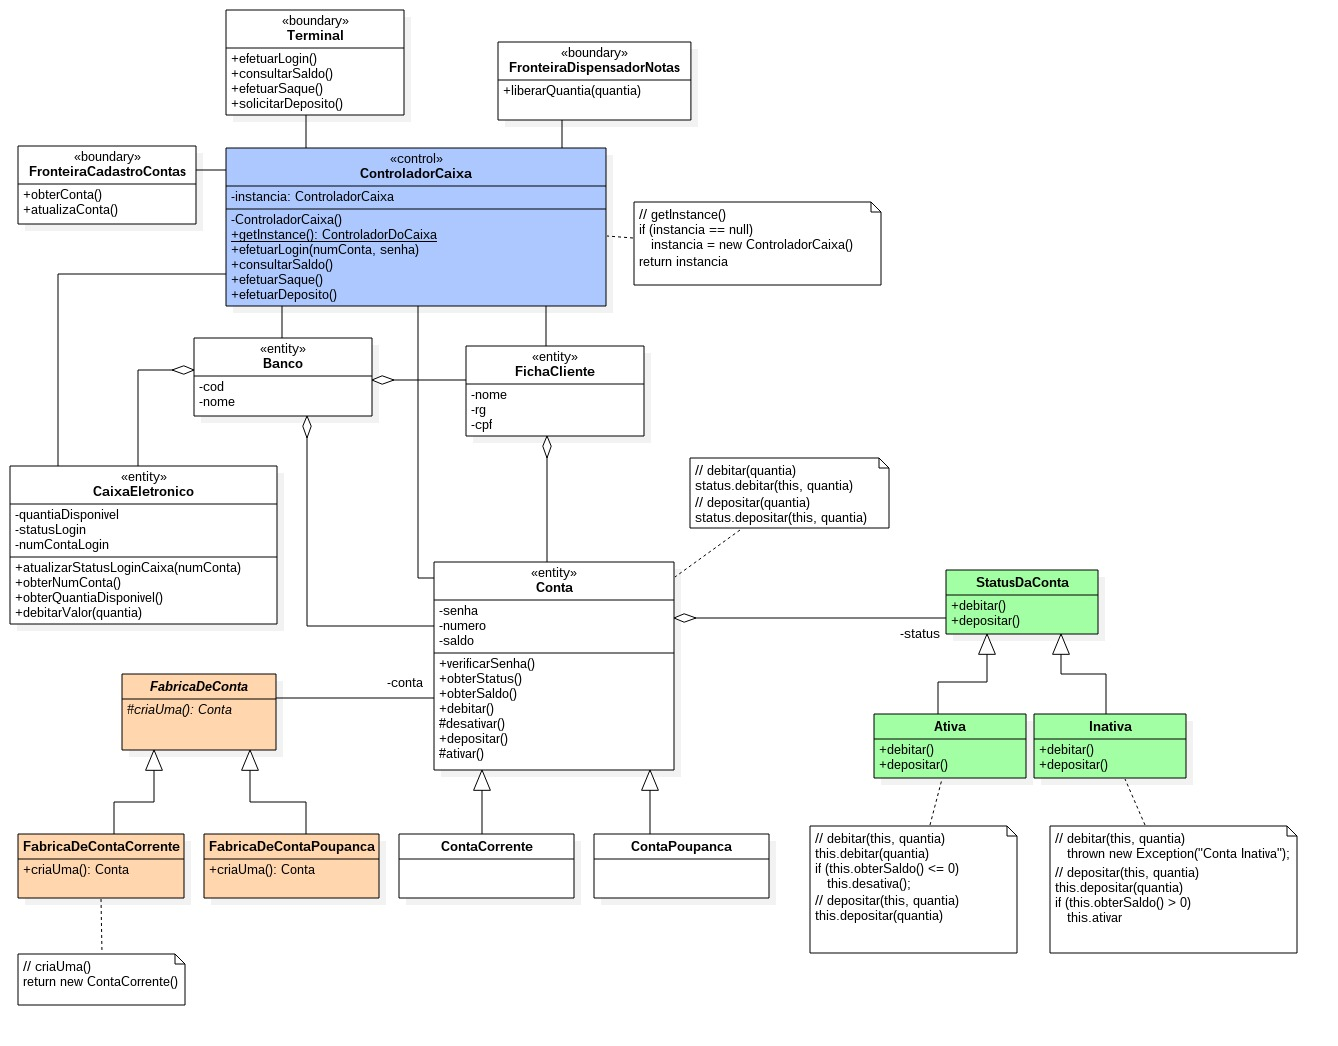
\includegraphics[width=0.92\textwidth]{imagens/lista2e3.jpg}
      \end{solution}
\pagebreak      
      \question Padrão de Projeto \textit{Façade}: aplique esse padrão definir componentes do sistema. 
      de contas.
      \begin{solution}
        A Interface do Padrão \textit{Façade} está destacadas em Cinza e o as classes do Padrão \textit{Factory Method}
        para instanciar o controlador estão destacadas em amarelo.
        
        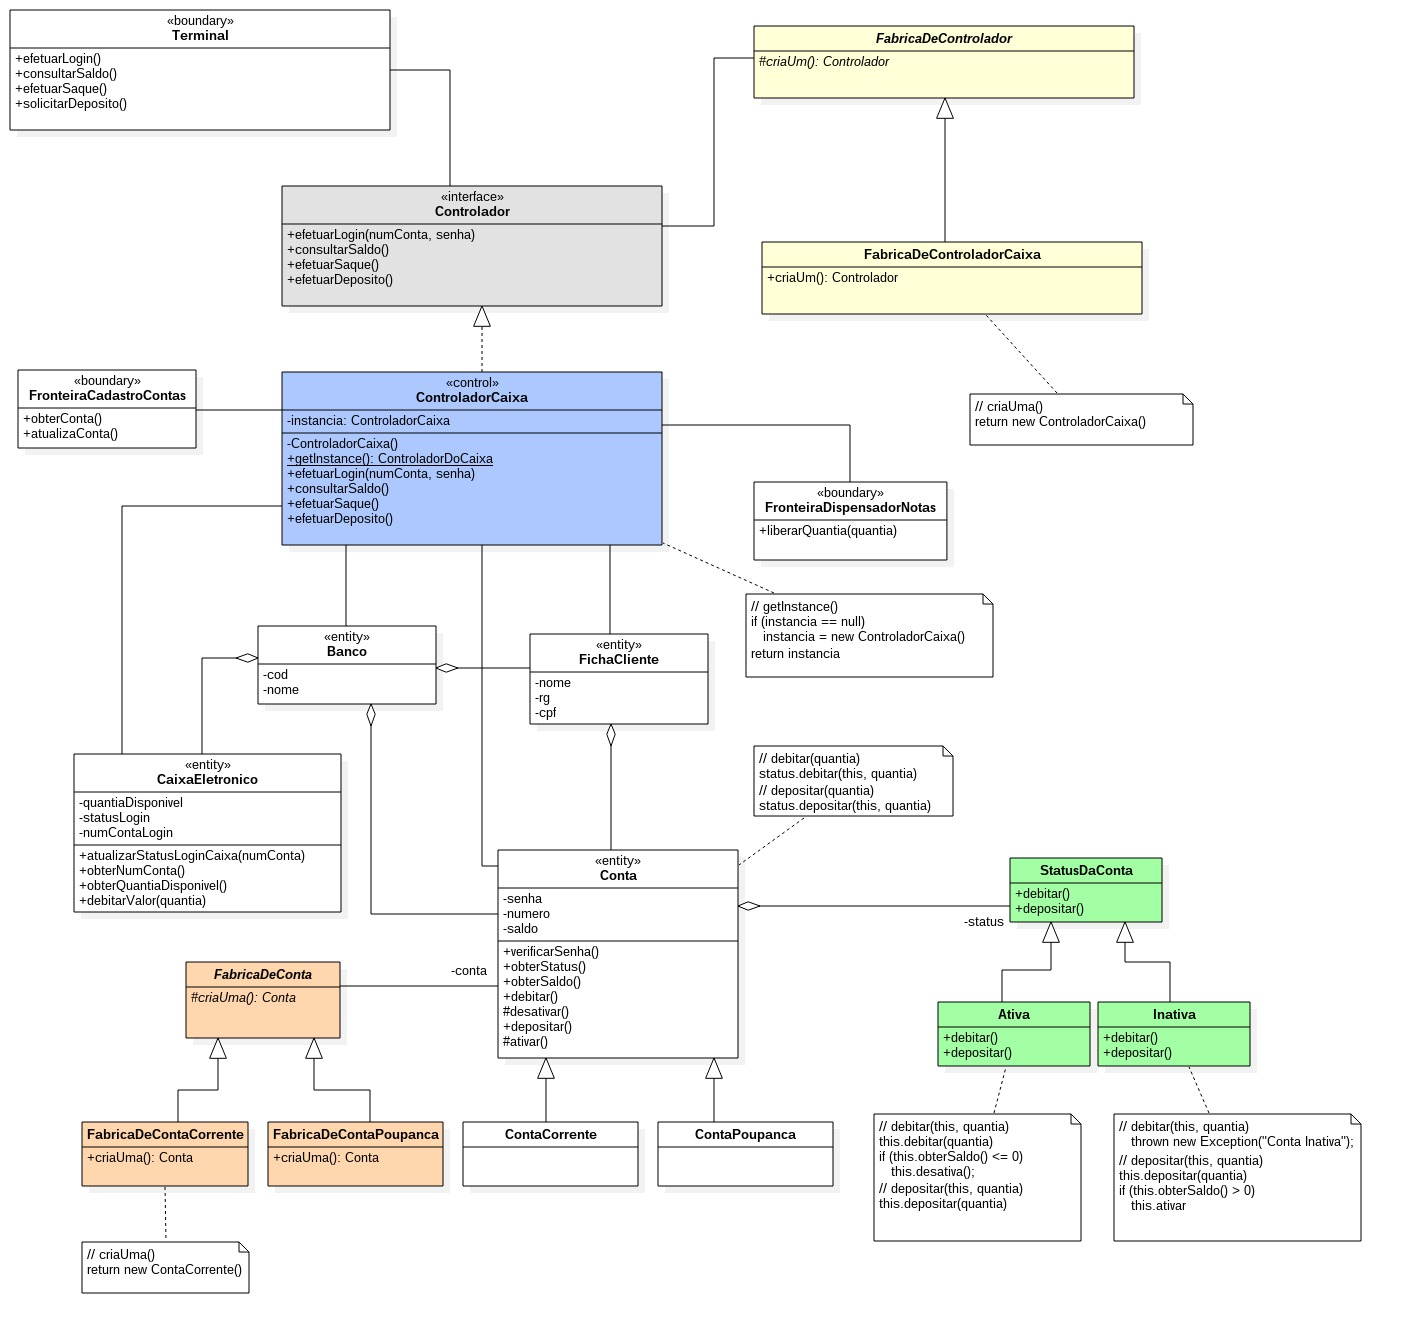
\includegraphics[width=0.82\textwidth]{imagens/lista2e4.jpg}
      \end{solution}
	
  \end{questions}

\end{document}
